\chapter{Physical Quantities}

\section{Units of measurement}

Any physical quantity contains a numerical value and its associated unit. The system of units of measurement used throughout the scientific world is the \keypoint{SI units}\index{SI unit}\footnote{SI units, abbreviated from the French \emph{Syst\`eme Internationale d'Unit\'es}, means the International System of Units. Those who are interested in the history and evolution of the SI can check out the Wikipedia article: \url{https://en.wikipedia.org/wiki/International_System_of_Units}}

\subsection{SI base units}

SI defines seven units of measure as a basic set, known as the \keypoint{SI base units}

\begin{center}
	\begin{tabular}{|C{5.4cm}|C{3cm}|C{3cm}|}
		\hline base quantity & base unit & symbol  \\ 
		\hline mass  & kilogram & kg \\ 
		\hline length & metre & m \\ 
		\hline time & second & s \\ 
		\hline electric current  & ampere & A \\ 
		\hline temperature & kelvin & K \\ 
		\hline amount of substance & mole & mol \\ 
		\hline luminous intensity & candela & cd \\ 
		\hline 
	\end{tabular} 
\end{center}


\subsection{Derived units}

The seven\footnote{Luminous intensity is beyond the scope of the A-Level syllabus. You are only required to know the other six SI base quantities and their units.} SI base units are building blocks of the SI system, all other quantities are derived from the base units.

\newpage

\example{Give the SI base units of (a) speed, (b) acceleration, (c) force, (d) work done.}
\begin{soln}
 $\text{speed} = \frac{\text{distance}}{\text{time}} \RA [v] = \frac{[s]}{[t]} = \frac{\text{m}}{\text{s}} = \text{m s}^{-1}$
	\end{soln}
 \begin{soln}
	$\text{acceleration} = \frac{\text{speed}}{\text{time}} \RA [a] = \frac{[v]}{[t]} = \frac{\text{m s}^{-1}}{\text{s}} = \text{m s}^{-2}$ 
\end{soln}
 \begin{soln}
	$\text{force} = \text{mass} \times \text{acceleration} \RA [F] = [m][a] = \text{kg}\mpss $5
	\end{soln}
 \begin{soln}
	$\text{work} = \text{force} \times \text{distance} \RA [W] = [F][s] = \text{kg}\mpss \times \text{m} = \text{kg m}^2 \text{s}^{-2}$ 
\end{soln}


\subsection{Metric prefixes}

To save writing so many figures, prefixes are used to indicate multiples and sub-multiples of original units

\begin{center}
	\begin{tabular}{|C{1.5cm}|C{1.5cm}|C{1.5cm}||C{1.5cm}|C{1.5cm}|C{1.5cm}|}
		\hline name & symbol & meaning & name & symbol & meaning \\ 
		\hline pico & p & $10^{-12}$ & hecto & h & $10^{2}$\\ 
		\hline nano & n & $10^{-9}$ & kilo & k & $10^{3}$\\ 
		\hline micro & $\mu$ & $10^{-6}$ & mega & M & $10^{6}$\\ 
		\hline milli & m & $10^{-3}$ & giga & G & $10^{9}$\\ 
		\hline centi & c & $10^{-2}$ & tera & T & $10^{12}$\\ 
		\hline deci & d & $10^{-1}$ & & &\\ 
		\hline 
	\end{tabular} 
\end{center}
\example{Alternative units of measurement for length}

	The radius of the Earth is about 6,370 km.
	
	The width of a human hair is around 60 $\sim$ 90 $\mu$m.
	
	The diameter of a water molecule is about 0.3 nm.
	
	The atomic radius of oxygen is about 60 pm. 

\subsection{Dimensional analysis}

\begin{ilight}
	If an equation is correct, then the units on both sides must be the same. An equation with consistent units is said to be \keypoint{homogeneous}.
\end{ilight}

\emph{Dimensional analysis} is widely used as a rough guide to check for the correctness of equations\index{dimensional analysis}. There are times when the dependence of one physical quantity on various other quantities cannot not be seen easily, but it might give us helpful hints by merely investigating their units.\\
There are \emph{unit free}, or \emph{dimensionless} quantities that do not have units. Examples of these are real numbers (2, $\frac{4}{3}$, $\pi$, etc.), coefficient of friction ($\mu$), refractive index ($n$), etc. \footnote{Note a correct equation must be homogeneous, but the converse may not be true. Possible problems include an incorrect coefficient, extra term, an incorrect sign, etc.}

\example{A ball falls in vacuum, all its gravitational potential energy converts into kinetic energy. This is expressed by the equation: $mgh = \frac{1}{2}mv^2$. Show that this equation is homogeneous.}
\begin{soln}
 LHS: $[mgh]=[m][g][h] = \text{kg} \times \mpss \times \text{m} = \text{kg m}^2\text{s}^{-2}$
	
	RHS: $\left[\frac{1}{2}mv^2\right] = [m][v]^2 = \text{kg} \times (\mps)^2 = \text{kg m}^2\text{s}^{-2}$
	
	so we see the equation $mgh = \frac{1}{2}mv^2$ is homogeneous \end{soln}
	
\example{The speed of a wave travelling along an elastic string is determined by three things: the tension $T$ in the string, the length $L$ of the string, and the mass $m$ of the string. Let's assume $v=T^a L^b m^c$, where $a$, $b$, $c$ are some numerical constants. Find the values of $a$, $b$ and $c$.}

\begin{soln} RHS: $[T]^a [L]^b [m]^c = (\text{kg m s}^{-2})^a \text{m}^b \text{kg}^c = \text{kg}^{a+c} \text{m}^{a+b} \text{s}^{-2a}$

for the equation to be homogeneous, we must have:
\begin{equation*}
	\text{kg}^{a+c} \text{m}^{a+b} \text{s}^{-2a} = \text{m s}^{-1} \RA
	\left\{ \begin{array}{ll}
	\text{kg}: & a+c=0 \\
	\text{m}: & a+b=1 \\
	\text{s}: & -2a=-1 \\
	\end{array}\right.
	\RA \left\{ \begin{array}{l}
	a=\tfrac{1}{2} \\
	b=\tfrac{1}{2} \\
	c=-\tfrac{1}{2} \\
	\end{array}\right.
\end{equation*}

so wave speed is given by: $v = T^{\sfrac{1}{2}} L^{\sfrac{1}{2}} m^{-\sfrac{1}{2}}$, or $v=\sqrt{\frac{TL}{m}}$

this happens to be the correct formula for the wave speed on a string \end{soln}


%\example{Evaluating how fast a man runs}
%	
%	Imagine an earth civilian was slaughtered by an alien army,  and his dead body was taken to the alien scientists. How can the alien tell how fast an average earthling runs?
%	
%	The speed $v$ at which a man runs may depend on 
%	
%	\exitem mass $m$ (fat people run more slowly)
%	
%	\exitem height $h$ (tall people have certain advantages in running)
%	
%	\exitem gravitational acceleration constant $g$ (think about the astronauts on the moon!)
%	
%	We know that $[m]=\text{kg}$, $[h]=\text{m}$, $[g]=\mpss$. The combination of these three quantities must give the same unit as $[v]=\mps$. Let's assume $v=m^a h^b g^c$, then we have $\text{m s}^{-1} = \text{kg}^a \text{m}^b \text{m}^c \text{s}^{-2c}$. We find the values for the constants $a=0$, $b=c=\frac{1}{2}$. So our best guess, the simplest construction to derive a quantity with the same unit as speed, is $v=\sqrt{gh}$.
%	
%	Let's estimate the speed of a 1.6 m tall boy with this formula: $v \approx \sqrt{10 \times 1.6} \approx 4 \tspace \mps$.
%	
%	It takes over 4 minutes for him to complete a 1 km trial. Despite being a crude model, it does make sense! \end{soln}
	



\subsection{Scalars \& Vectors}

Physical quantities come in two types: scalars and vectors.

\begin{ilight}
	a \keypoint{scalar} quantity has magnitude only
	
	a \keypoint{vector} quantity has magnitude and direction
\end{ilight}


In other words, a scalar can be described by a single number. Examples of scalars are	time, distance, speed, mass, temperature, energy, density, volume, etc.

\begin{marginfigure}
	\vspace{-10pt}
	\begin{center}
		\begin{tikzpicture}[scale=0.6]
		\draw[->] (0,0) node[left]{$A$} to node[midway,above]{$\overrightarrow{p}$} (4,2) node[right]{$B$};
		\end{tikzpicture}
	\end{center}
	\vspace{-27pt}
\end{marginfigure}


A vector, on the other hand, is usually represented by an arrow in a specific direction. A vector $\overrightarrow{p}$ pointing from $A$ to $B$ is shown. The length of the arrow shows the magnitude of the vector, the direction of the arrow gives the direction of the vector. Examples of vectors are	displacement, velocity, acceleration, force, field strength, etc.	

\subsection{Adding Vectors}
Scalar algebra is just ordinary algebra - one can add and subtract scalar quantities in the same way as if they were ordinary numbers, for example, a set of objects with mass $m_1$, $m_2$, $\cdots$, $m_n$ have a total mass of $M=m_1+m_2+\cdots+m_n$ 


Vector algebra on the other hand is more complicated, since we need keep track of the direction \index{vector algebra}

Vectors can be added to form a \keypoint{resultant} vector - to deal with vector sums, we need take the directions of vectors into account.

Let's consider the sum of two vectors $\overrightarrow{p_1}$ and $\overrightarrow{p_2}$:

The resultant vector $\overrightarrow{p} = \overrightarrow{p_1} + \overrightarrow{p_2}$ lies on diagonal of the parallelogram subtended by $\overrightarrow{p_1}$ and $\overrightarrow{p_2}$, this is called the \keypoint{parallelogram rule} for vector addition. If the resultant of several vectors $\overrightarrow{p} = \overrightarrow{p_1} + \overrightarrow{p_2} + \cdots \overrightarrow{p_n}$ is to be found, one can join these vectors head-to-tail, the resultant is given by the arrow connecting the tail of $\overrightarrow{p_1}$ to the head of $\overrightarrow{p_n}$:

\begin{figure}[ht]
		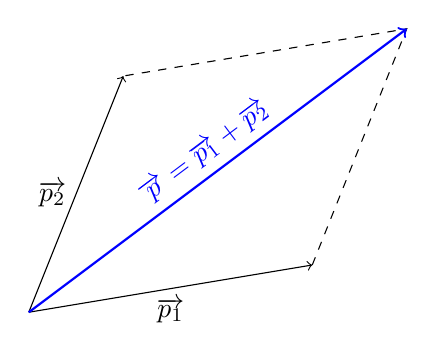
\begin{tikzpicture}[scale=1.2]
		\draw[->] (0,0) -- (3,0.5) node[midway,below]{$\overrightarrow{p_1}$};
		\draw[->] (0,0) -- (1,2.5) node[midway,left]{$\overrightarrow{p_2}$};
		\draw[dashed] (3,0.5) -- (4,3) -- (1,2.5);
		\draw[thick, ->, blue] (0,0) -- (4,3) node[midway,above,rotate=36.87]{$\overrightarrow{p} = \overrightarrow{p_1} + \overrightarrow{p_2}$};
		\end{tikzpicture}
 \end{figure}
 \begin{figure}
		\centering
		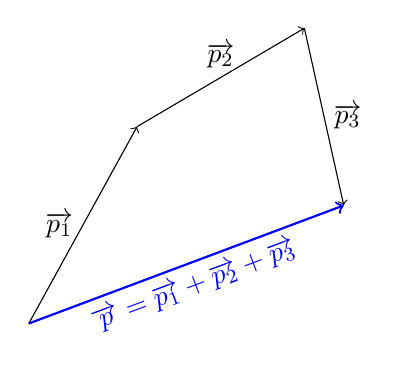
\begin{tikzpicture}[scale=1.25]
		\draw[->] (0,0) -- (1.1,2) node[midway,left]{$\overrightarrow{p_1}$};
		\draw[->] (1.1,2) -- (2.8,3) node[midway,above]{$\overrightarrow{p_2}$};
		\draw[->] (2.8,3) -- (3.2,1.2) node[midway,right]{$\overrightarrow{p_3}$};
		\draw[thick, ->, blue] (0,0) -- (3.2,1.2) node[midway,below,rotate=20.556]{$\overrightarrow{p} = \overrightarrow{p_1} + \overrightarrow{p_2} + \overrightarrow{p_3}$};
		\end{tikzpicture}
\end{figure}

\example{A river flows from south to north with a speed of $2.0 \mps$ and the speed of a boat with respect to the water flow is $5.0 \mps$. (a) Suppose the boat leaves the west bank heading due east, what is the resultant velocity of the boat? (b) If the boat is to reach the exact opposite bank across the river, what is the resultant velocity and in what direction should the boat be headed?}

\begin{soln} Vector diagrams for the resultant velocity of the boat are illustrated below for part (a) boat heading due south:

magnitude of resultant velocity: $v = \sqrt{v_b^2 + v_w^2} = \sqrt{5.0^2 +2.0^2} \approx 5.4 \mps$.

In this case, the boat reaches opposite bank in shortest time but will drift downstream.
\end{soln}
\begin{figure}
		\centering
		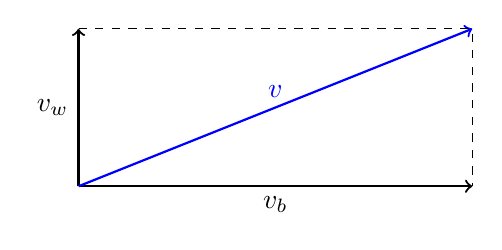
\begin{tikzpicture}
		\draw[thick,->] (0,0) -- (0,2) node[midway,left]{$v_w$};
		\draw[thick,->] (0,0) -- (5,0) node[midway,below]{$v_b$};
		\draw[thick,blue,->] (0,0) -- (5,2) node[midway,above]{$v$};
		\draw[dashed] (0,2) -- (5,2) -- (5,0);
		\end{tikzpicture}
		
\end{figure}		
\begin{soln}
For part (b), the boat is to hit the opposite bank:
magnitude of resultant velocity: $v = \sqrt{v_b^2 + v_w^2} = \sqrt{5.0^2 -2.0^2} \approx 4.6 \mps$. in this case, the boat reaches opposite bank in shortest distance but the boat is headed slightly upstream: $\theta = \sin^{-1} \frac{v_w}{v_b} = \sin^{-1}\frac{2.0}{5.0} \approx 24^\circ$
\end{soln}		
  
\begin{figure}	
		\centering
		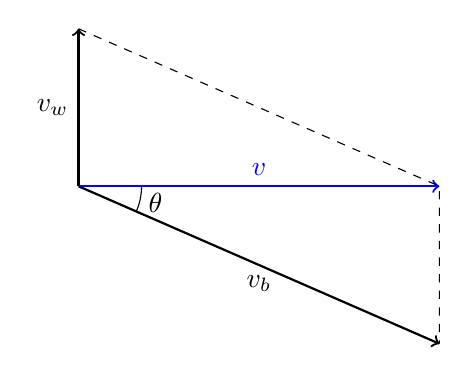
\begin{tikzpicture}
		\draw[thick,->] (0,0) -- (0,2) node[midway,left]{$v_w$};
		\draw[thick,->] (0,0) -- (4.583,-2) node[midway,below]{$v_b$};
		\draw[thick,blue,->] (0,0) -- (4.583,0) node[midway,above]{$v$};
		\draw[dashed] (0,2) -- (4.583,0) -- (4.583,-2);
		\draw (0.8,0) arc(0:-23.58:0.8);
		\node at (-12:1) {$\theta$};
		\end{tikzpicture}
\end{figure}


\subsection{Multiplication of vectors}

Vectors can be multiplied by scalars easily, 
\footnote{It is also possible to multiply vectors with vectors, but we'll not go this far in A-level Physics. There are basically two ways of doing vector multiplication: the \emph{dot product} and the \emph{cross product}. Both vector products are useful in physics, but we will not go into the details. You will learn more about vector multiplication in the A-Level mathematics course.\piste} when being multiplied by a scalar number, magnitude of the vector changes. If this number is positive, the vector becomes longer or shorter, but still points in same direction, if the number to be multiplied is negative, the operation reverses the vector's direction...

\example{Given a vector $\overrightarrow{p}$, the graphical representations of $2\overrightarrow{p}$, $\frac{1}{2}\overrightarrow{p}$, $-\overrightarrow{p}$, $-\frac{3}{2}\overrightarrow{p}$ are:}
\begin{figure*}
\begin{center}
    

	\begin{tikzpicture}[scale=.8]
	\draw[->] (0,-2.5) node{$\overrightarrow{p}$} (-1,-1) -- (1,1);
	\draw[->] (4,-2.5) node{$2\overrightarrow{p}$} (2,-2) -- (6,2);
	\draw[->] (8,-2.5) node{$\frac{1}{2}\overrightarrow{p}$} (7.5,-.5) -- (8.5,.5);
	\draw[->] (12,-2.5) node{$-\overrightarrow{p}$} (13,1) -- (11,-1);
	\draw[->] (16,-2.5) node{$-\frac{3}{2}\overrightarrow{p}$} (17.5,1.5) -- (14.5,-1.5);
	\end{tikzpicture}
 \end{center}
\end{figure*}	

\subsection{Resolving vectors}

Just as it's useful to combine two vectors into a resultant, one can also resolve a single vector into two (or more) components.
\footnote{This depends on the number of dimensions of space we are working with.}

Lets draw an arbitrary 2D vector and call it $\overrightarrow{p}$:
\begin{figure}
	\vspace{-18pt}
	\begin{center}
		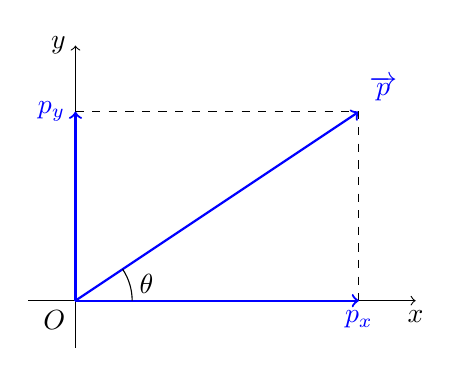
\begin{tikzpicture}[scale=1.2]
		\draw[->] (-.5,0) -- (3.6,0) node[below]{$x$};
		\draw[->] (0,-.5) -- (0,2.7) node[left]{$y$};
		\draw[thick, ->, blue] (0,0) node[below left]{\textcolor{black}{$O$}} -- (3,2) node[above right]{$\overrightarrow{p}$};
		\draw[dashed] (0,2) -- (3,2) -- (3,0);
		\draw[thick, ->, blue] (0,0) -- (0,2) node[left]{$p_y$};
		\draw[thick, ->, blue] (0,0) -- (3,0) node[below]{$p_x$};
		\draw (0:0.6) arc [radius=0.6, start angle=0, end angle= 33.7] node[midway,right]{$\theta$};
		\end{tikzpicture}
	\end{center}
	\vspace{-25pt}
\end{figure}
You can hopefully see here how the vector $\overrightarrow{p}$ can be split into two perpendicular components:

\titem a horizontal component $p_x$

\titem a vertical component $p_y$

Given that $\overrightarrow{p}$ forms an angle $\theta$ to the $x$-axis, then:
$$p_x = p \cos \theta$$ $$p_y = p \sin \theta$$
$$p = |\overrightarrow{p}| = \sqrt{p^2_x + p^2_y}$$,
$$\quad\tan \theta = \frac{p_y}{p_x}$$
	

\newpage

\example{A force of 3.0 N towards east and a force of 2.0 N towards 30$^\circ$ north of east act on an object. Find the magnitude and the direction of the resultant force.}


\begin{soln} suppose an arrow of length 1 cm represents a force of 1 N

one can draw a \emph{scale diagram} with a ruler and a protractor as shown
\end{soln}
\begin{figure}[ht]
	\centering
	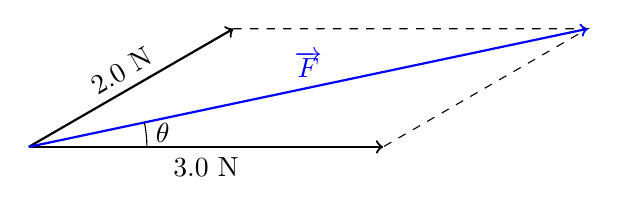
\begin{tikzpicture}[scale = 1.5]
	\draw[thick,->] (0,0) -- (3,0) node[midway,below]{3.0 N};
	\draw[thick,->] (0,0) -- ++ (30:2) node[midway,above,rotate=30]{2.0 N};
	\draw[dashed] (30:2) --++ (3,0) --++ (-150:2);
	\draw[thick,blue,->] (0,0) -- (4.732,1) node[midway, above]{$\overrightarrow{F}$};
	\draw (1,0) arc(0:11.9:1);
	\node at (1.135, 0.12) {$\theta$};
	\end{tikzpicture}
\end{figure}

\begin{soln}
one can find length of the resultant vector is about 4.8 cm

also it forms an angle of about 12$^\circ$ to the 3.0 N force

so resultant force is of 4.8 N acting towards 12$^\circ$ north of east

alternatively, one can find components of the resultant as the sum of individual components

{
	\centering
	
	$F_x = 3.0 + 2.0 \cos 30^\circ \approx 4.73 \text{ N}, \quad F_y = 2.0\sin30^\circ = 1.0 \text{ N}$
	
}

magnitude and direction of the resultant can then be found from its components

{
	\centering
	
	$F = \sqrt{F_x^2 + F_y^2} = \sqrt{4.73^2 + 1.0^2} \approx 4.84 \text{ N}, \theta = \tan^{-1}\frac{F_y}{F_x} = \tan^{-1}\frac{1.0}{4.73} \approx 11.9^\circ$
	
}

this of course agrees with scale diagram method, but resolving gives more precise results \end{soln}

\begin{marginfigure}
	\vspace*{-10pt}
	\centering
	\begin{tikzpicture}[scale=1.1]
	\draw[thick] (0,0) -- (30:5) -- ++(0,-2.5) -- cycle;
	\draw[thick] (0.8,0) arc(0:30:0.8);
	\node at (15:1) {$\theta$};
	\draw[thick] (30:2.5) -- ++(120:1) -- ++(30:1) -- ++(-60:1);
	\draw[thick] (-1,0) -- (5,0);
	\draw[thick,->] (2.348,1.933) --++ (0,-1.6) node[right,pos=0.7]{$W$};
	\draw[thick,blue,->] (2.348,1.933) --++ (210:0.8) node[left]{$W_\parallelslant$};
	\draw[thick,blue,->] (2.348,1.933) --++ (-60:1.38564) node[right]{$W_\perp$};;
	\draw[dashed] (2.348,1.933) ++ (210:0.8) --++ (-60:1.38564) --++ (30:0.8) ;
	\end{tikzpicture}
	\vspace*{-16pt}
\end{marginfigure}


\example{A box of weight $W=20.0 \text{ N}$ is resting on an inclined slope at 30$^\circ$ to the horizontal. Find the components of weight parallel to the slope and normal to the slope.}\label{ex:comp-of-W}

\begin{soln} the vector diagram is shown

component of weight parallel to slope: $W_\parallelslant = W\sin\theta = 20.0\times \sin30^\circ = 10.0 \text{ N}$

component of weight normal to slope: $W_\perp = W\cos\theta = 20.0\times \cos30^\circ \approx 17.3 \text{ N}$ \end{soln}


	
\subsection{Questions}

\subsection*{SI units}

\question{What are the SI base units of (a) density, (b) pressure, (c) energy, (d) electric charge?}

\question{For a substance of mass $m$, the heat energy $Q$ needed to change its temperature by $\Delta T$ is given by: $Q = cm\Delta T$. Find the SI base units of the constant $c$.}

\subsection*{Dimensional analysis}

\question{The resistive force $F$ on a metal ball falling at low speeds in water is given by the equation $F = krv$, where $r$ is the radius of the metal ball, $v$ is its speed and $k$ is a constant.
	Find the base units of $k$ in the SI system.}

\question{The speed of sound in air can be given by $c=\sqrt{\frac{\gamma p}{\rho}}$, where $p$ is the pressure of the air and $\rho$ is the air density. Show that $\gamma$ is unit free.}

\question{The effective power output from a wind turbine is given by the equation $P = \frac{1}{2} \eta \rho A v^n$, where $\rho$ is the air density, $A$ is the area of the turbine blades, and $v$ is the wind speed. Given that $\eta$ is a constant with no units, what is the value of $n$?}

\subsection*{Vector algebra}

\question{An aircraft, which has a speed of $35 \mps$ in still air, is flying from south to north at a speed of $32 \mps$ with respect to a stationary observer on the ground. Find the magnitude and the possible directions of wind velocity.}

\question{Three forces of 5.0 N, 12 N and 13 N act at one point on an object. The angles at which the forces act can vary. What is the maximum and the minimum resultant force?}


